{
{\sffamily Her præsenteres forslag til forbedringer til vores
implementation og analyse.
}

\begin{itemize}
    \item Bedre udtrækning af regioner
    \item Selv implementere floodfill, så vi kan få gemt nogle flere
    dataer om ragionerne under vejs, så vi ikke behøver at lave gridt
    over billedet.
    \item Mere sofistikeret valg af tilfældig farve.
    \item Unikke regioner i databasen/analysen.
    \item Gyldne snit i de enkelte regioner.
    \item Gemme alle interessante regioner fra en analyse.
\end{itemize}

\subsection{Vurdering af regioner}
Vi ser her på mulige forbedringer ved vurdering af regioner.  Vi har i
tidligere afsnit, været inde på, hvilke mangler vores nuværende metoder
har, og vi vil derfor komme ind på følgende forslag:
\begin{enumerate}
    \item Eventuel sammensmeltning af naiv og udvidet løsning
    \item Pointscore i stedet for binær klassifikation
    \item Bonus for regioner som ligger i flere gyldne snit
    \item Ligger der interessante regioner i ``Eye of God''?
    \item ``Skæve'' snit, dvs. diagonaler og arbitrære snit.
    \item Er en fundet region, malet efter det gyldne snit?
\end{enumerate}

De to første punkter udelukker til dels hinanden, for enten vælges nr.
1, hvor vi beholder den binære klassifikation, eller også bruges en helt
anden metode, som søger at give hver region points for hvorvidt denne
ligger i det gyldne snit. Vi ser det dog som et oplagt, og nødvendigt,
tiltag, at forlade den binære klassifikation og bruge en pointscore i
stedet. Vi har allerede givet et forslag til en sådan metode i afsnit
\ref{section_udvidelser}, hvor det blev foreslået at bruge et
topografisk kort, til at udregne omkostninger for regioner. Regionen
kunne approksimeres ved brug af et gitter eller dennes konvekse hylster.

Punkt nr. 3 er egentlig kun interessant, hvis man bruger pointscore til
regioner, da man ved en binær klassificering, ikke kan gøre en region
``mere godkendt''. Man kunne

\begin{figure}[!h]
    \centering
    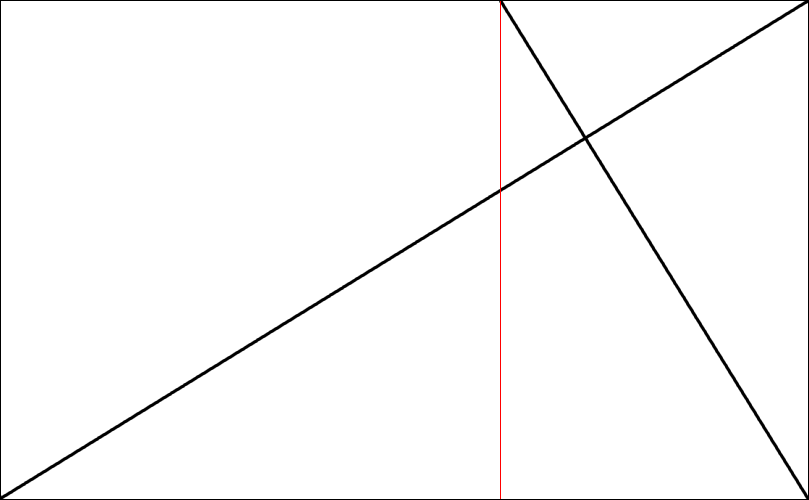
\includegraphics[angle=0,width=0.4\textwidth]{afsnit/fremtidigt_arbejde/billeder/eye_of_god}
    \caption[]{Punktet hvor de to sorte linjer krydser, kaldes ``The Eye
    of God'', og er her vist i et gyldent rektangel.}
    \label{eye_of_god}
\end{figure}

\subsection{Udtrækning af regioner}
\begin{enumerate}
    \item Bedre udtrækning af regioner.
    \item Selv implementere floodfill, så vi kan udtrække flere data om
        regionerne undervejs (så vi ikke behøver at lave gridt over
        billedet).
    \item Mere sofistikeret valg af tilfældig farve.
    \item Fuld segmentering af billedet.
    \item Unikke regioner i databasen/analysen.
\end{enumerate}

}

% vim: set tw=72 spell spelllang=da:
